\chapter{Resultados e discussão}
\label{chap:resultados}

Para apresentação dos resultados encontrados ao longo da implantação da mesa cartesiana no 
laboratório de sistemas térmicos e uma posterior discussão, os temas foram divididos de acordo 
com a metodologia (seção 3). Ou seja, primeiramente é apresentado os resultados do sistema mecânico, 
em seguida é mostrado os resultados da programação do sistema de software.

\section{Sistema mecânico}\label{sec:resmecanico}

A Figura X mostra uma fotografia da mesa cartesiana possibilitando uma melhor compreensão do funcionamento 
dos seus componentes.

% LANDSCAPE  - width = 0.4\linewidth
% LANDSCAPE  - scale = 0.30
% NORMAL  - width = 0.7\linewidth
% NORMAL  - scale = 0.45 a que eu mais gostei
%\begin{landscape}
\begin{figure}[H]
\centering
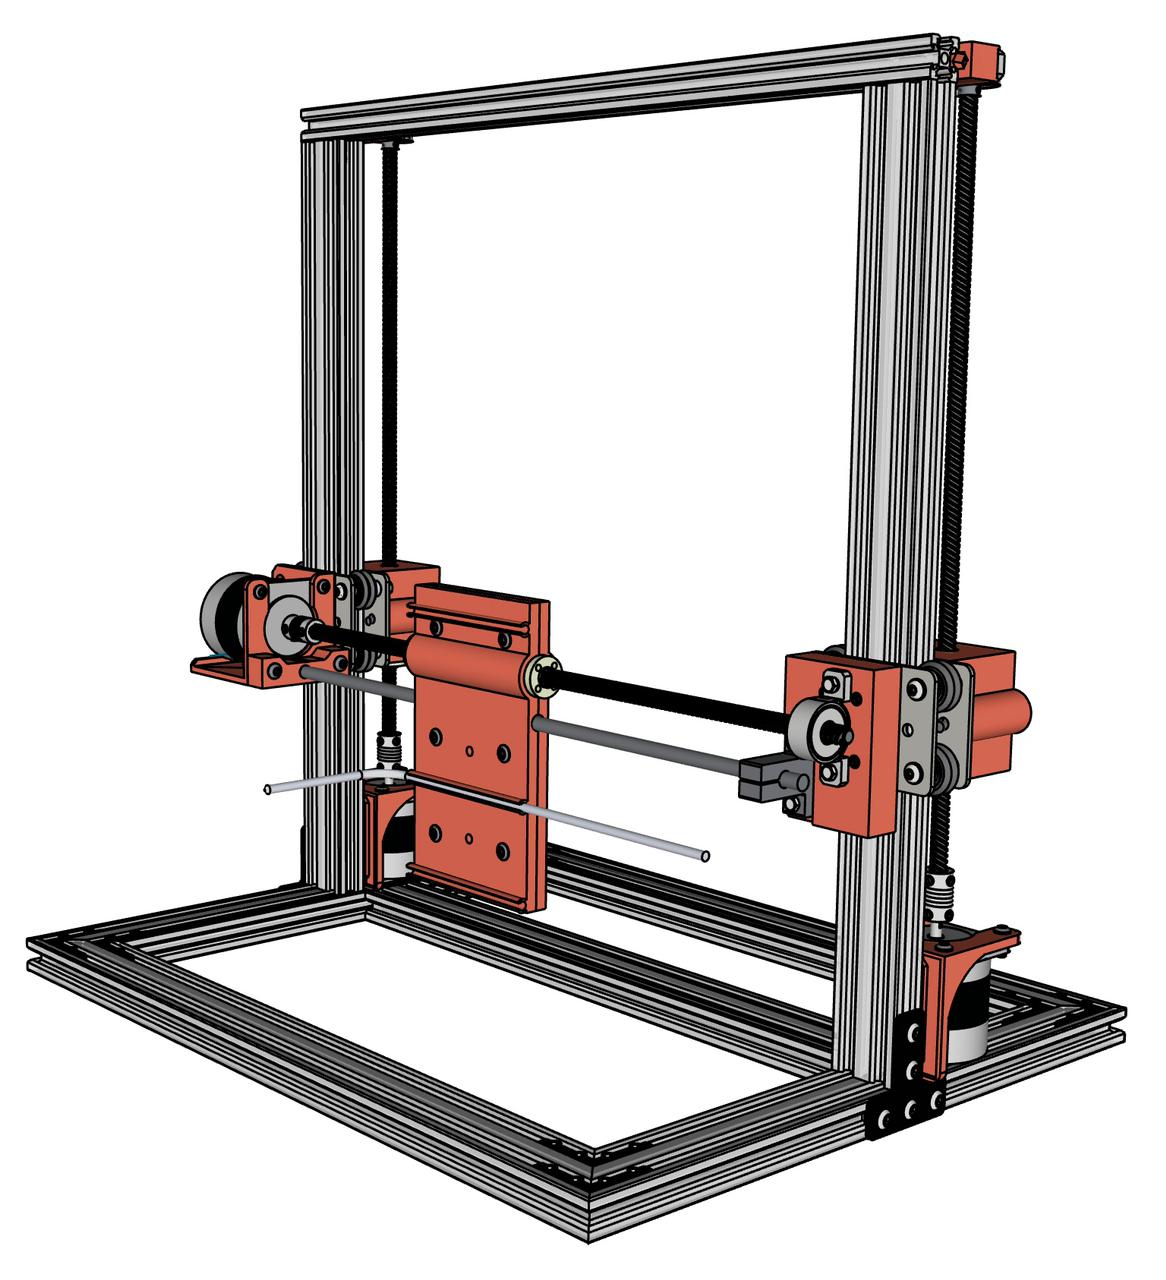
\includegraphics[scale = 0.35]{figuras/mesacartesianaperfil}
\caption{Sistema mecânico da mesa cartesiana vista de perfil.}
\caption*{Fonte: Próprio autor}
\label{fig:mesacartesianaperfil}
\end{figure}
%\end{landscape}

% LANDSCAPE  - width = 0.4\linewidth
% LANDSCAPE  - scale = 0.30
% NORMAL  - width = 0.7\linewidth
% NORMAL  - scale = 0.45 a que eu mais gostei
%\begin{landscape}
\begin{figure}[H]
\centering
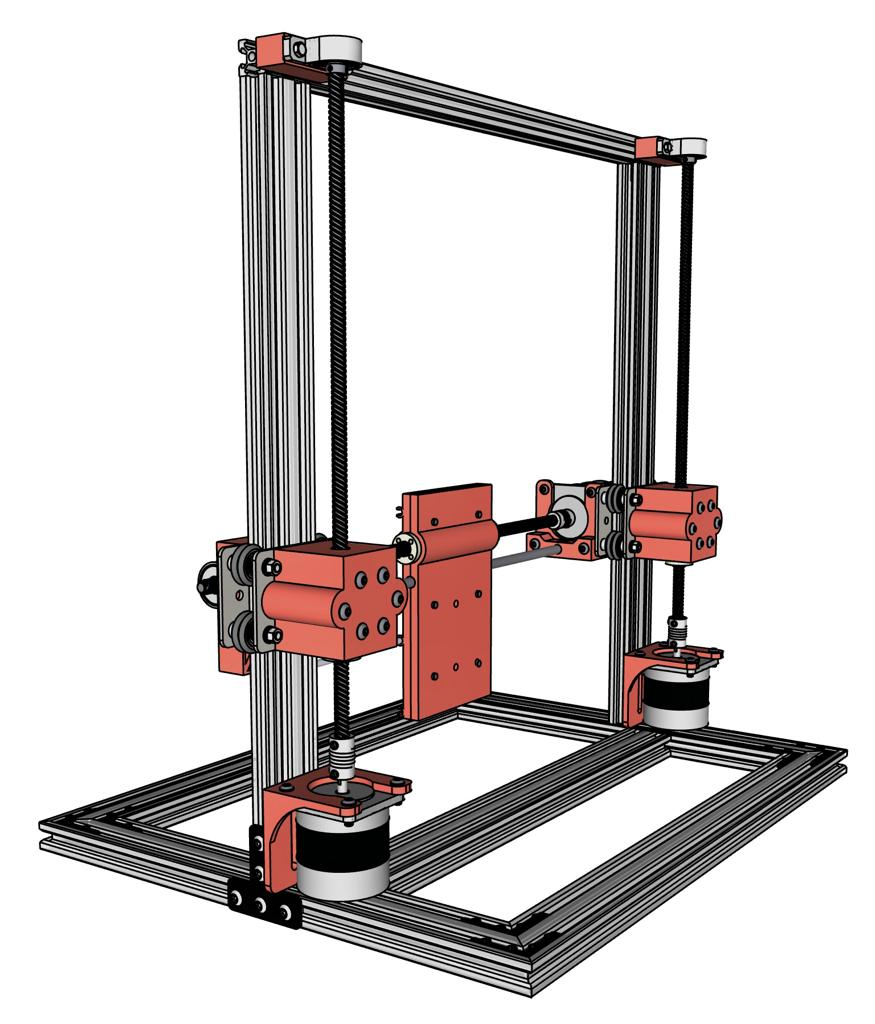
\includegraphics[scale = 0.35]{figuras/mesacartesianaperfiltraseira}
\caption{Sistema mecânico da mesa cartesiana vista de perfil traseira.}
\caption*{Fonte: Próprio autor}
\label{fig:mesacartesianaperfiltraseira}
\end{figure}
%\end{landscape}
        

% LANDSCAPE  - width = 0.4\linewidth
% LANDSCAPE  - scale = 0.30
% NORMAL  - width = 0.7\linewidth
% NORMAL  - scale = 0.45 a que eu mais gostei
%\begin{landscape}
\begin{figure}[H]
\centering
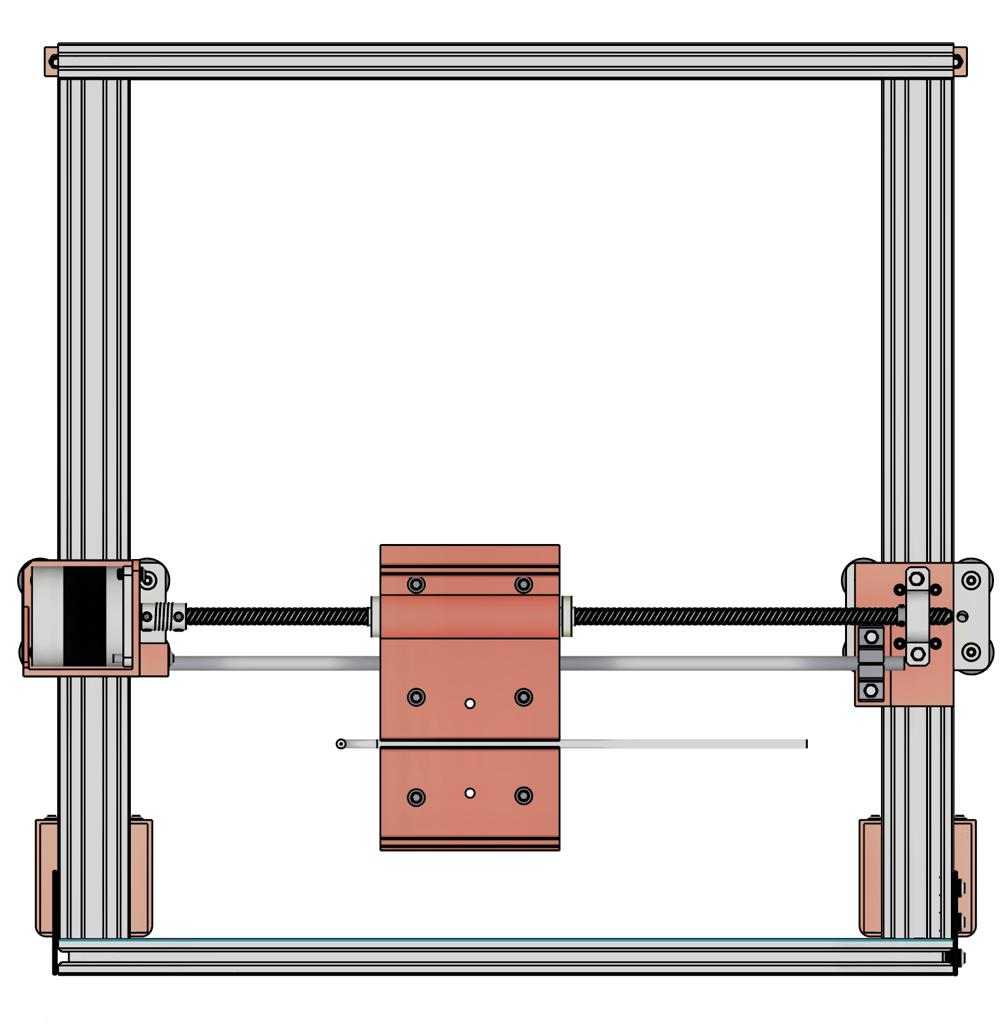
\includegraphics[scale = 0.25]{figuras/mesacartesianafrontal}
\caption{Sistema mecânico da mesa cartesiana vista frontal.}
\caption*{Fonte: Próprio autor}
\label{fig:mesacartesianafrontal}
\end{figure}
%\end{landscape}

% LANDSCAPE  - width = 0.4\linewidth
% LANDSCAPE  - scale = 0.30
% NORMAL  - width = 0.7\linewidth
% NORMAL  - scale = 0.45 a que eu mais gostei
%\begin{landscape}
\begin{figure}[H]
\centering
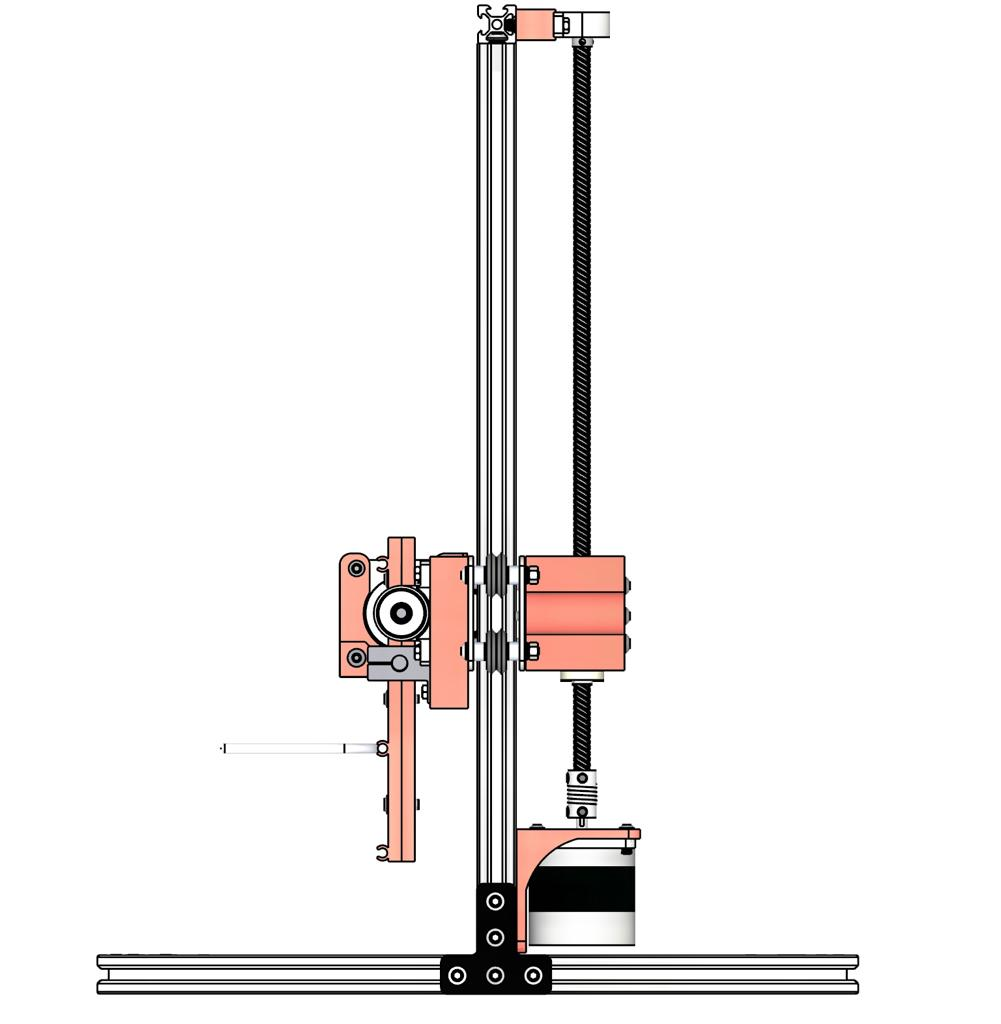
\includegraphics[scale = 0.25]{figuras/mesacartesianalateral}
\caption{Sistema mecânico da mesa cartesiana vista lateral.}
\caption*{Fonte: Próprio autor}
\label{fig:mesacartesianalateral}
\end{figure}
%\end{landscape}
        
% LANDSCAPE  - width = 0.4\linewidth
% LANDSCAPE  - scale = 0.30
% NORMAL  - width = 0.7\linewidth
% NORMAL  - scale = 0.45 a que eu mais gostei
%\begin{landscape}
\begin{figure}[H]
\centering
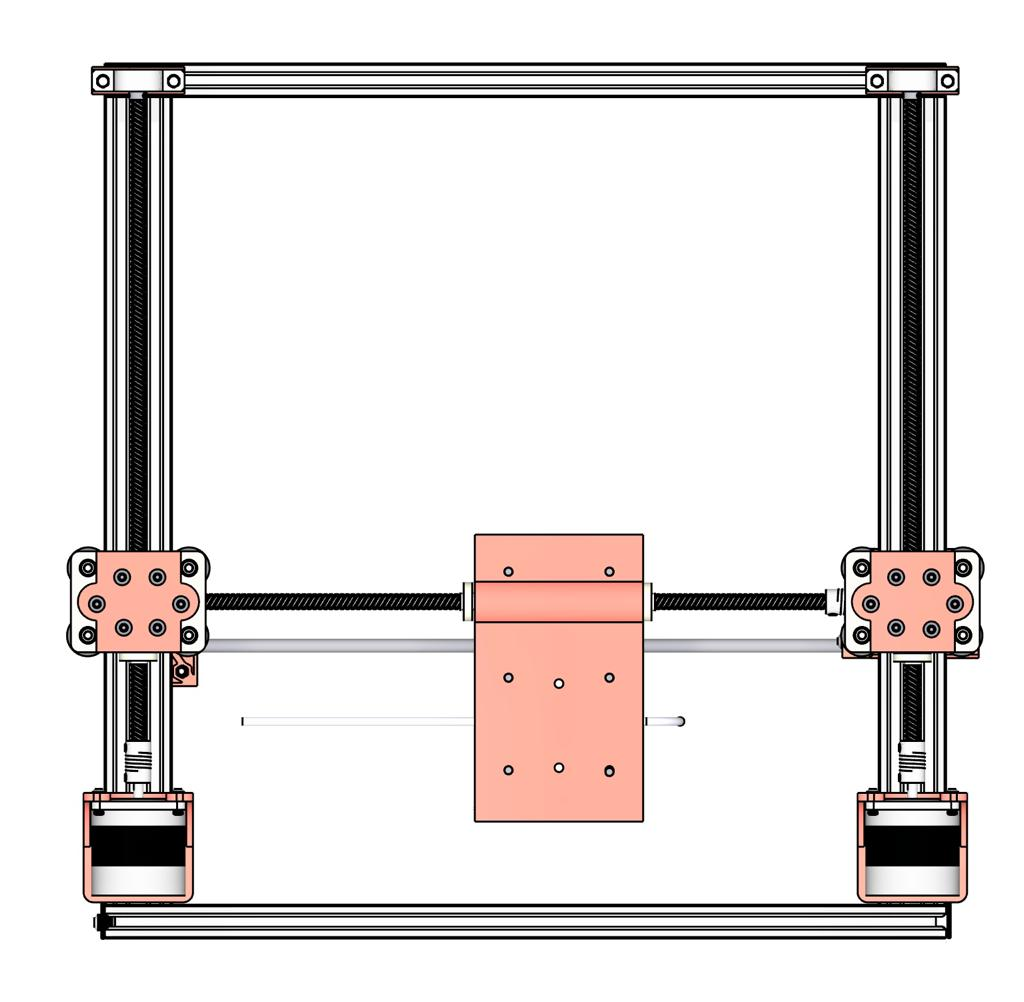
\includegraphics[scale = 0.25]{figuras/mesacartesianatraseira}
\caption{Sistema mecânico da mesa cartesiana vista traseira.}
\caption*{Fonte: Próprio autor}
\label{fig:mesacartesianatraseira}
\end{figure}
%\end{landscape}

% LANDSCAPE  - width = 0.4\linewidth
% LANDSCAPE  - scale = 0.30
% NORMAL  - width = 0.7\linewidth
% NORMAL  - scale = 0.45 a que eu mais gostei
%\begin{landscape}
\begin{figure}[H]
\centering
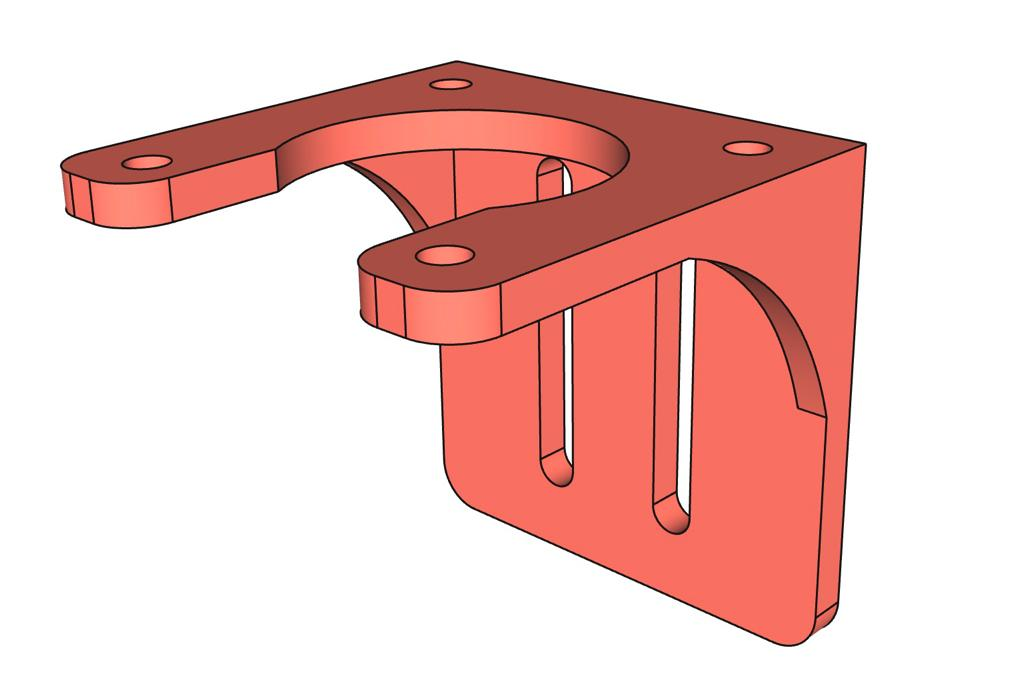
\includegraphics[scale = 0.4]{figuras/ressuportemotorpasso}
\caption{Suporte do motor de passo.}
\caption*{Fonte: Próprio autor}
\label{fig:ressuportemotorpasso}
\end{figure}
%\end{landscape}

% LANDSCAPE  - width = 0.4\linewidth
% LANDSCAPE  - scale = 0.30
% NORMAL  - width = 0.7\linewidth
% NORMAL  - scale = 0.45 a que eu mais gostei
%\begin{landscape}
\begin{figure}[H]
\centering
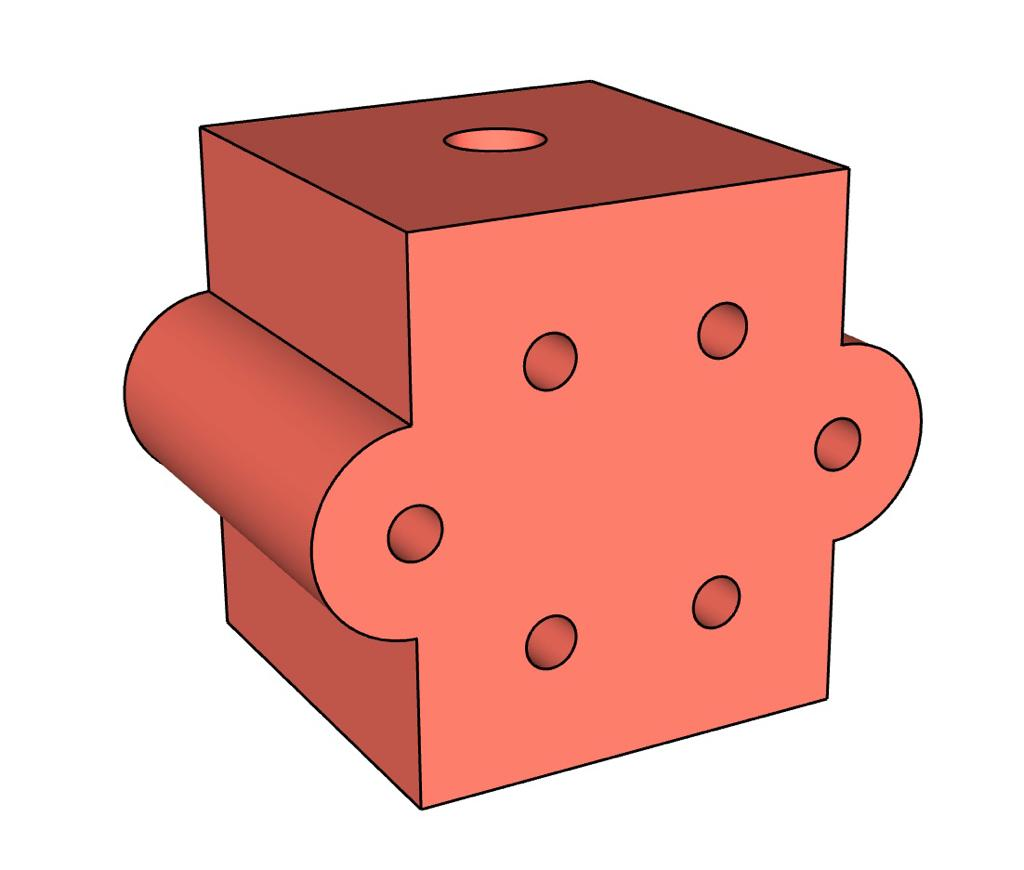
\includegraphics[scale = 0.4]{figuras/ressuporteelevacao}
\caption{Suporte de elevação.}
\caption*{Fonte: Próprio autor}
\label{fig:ressuporteelevacao}
\end{figure}
%\end{landscape}

% LANDSCAPE  - width = 0.4\linewidth
% LANDSCAPE  - scale = 0.30
% NORMAL  - width = 0.7\linewidth
% NORMAL  - scale = 0.45 a que eu mais gostei
%\begin{landscape}
\begin{figure}[H]
\centering
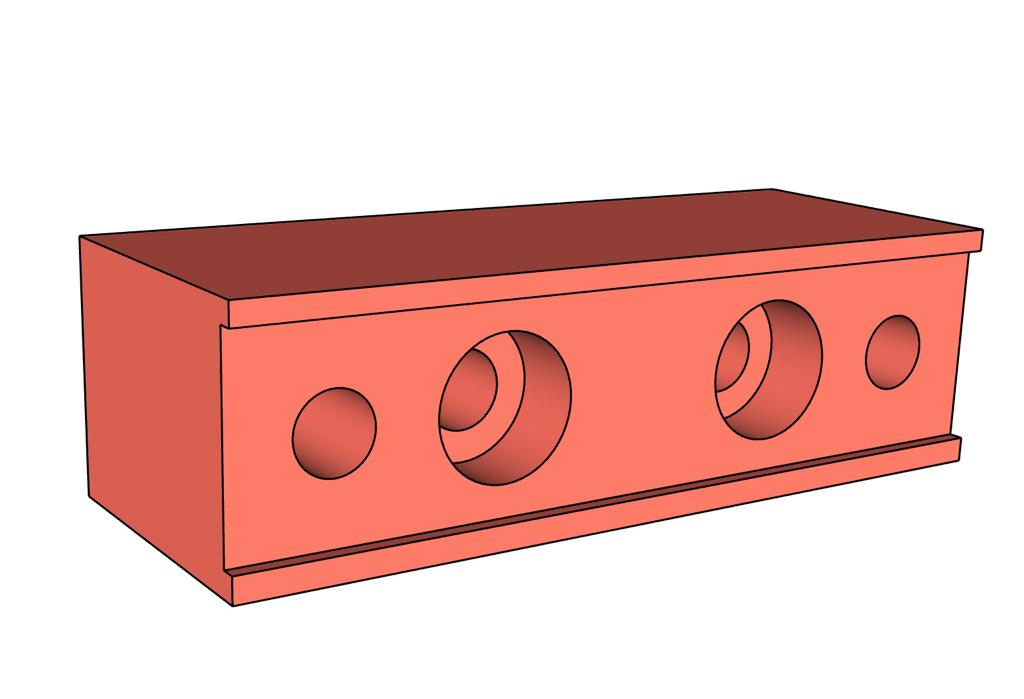
\includegraphics[scale = 0.4]{figuras/ressuportemancal}
\caption{Suporte do mancal.}
\caption*{Fonte: Próprio autor}
\label{fig:ressuportemancal}
\end{figure}
%\end{landscape}

% LANDSCAPE  - width = 0.4\linewidth
% LANDSCAPE  - scale = 0.30
% NORMAL  - width = 0.7\linewidth
% NORMAL  - scale = 0.45 a que eu mais gostei
%\begin{landscape}
\begin{figure}[H]
\centering
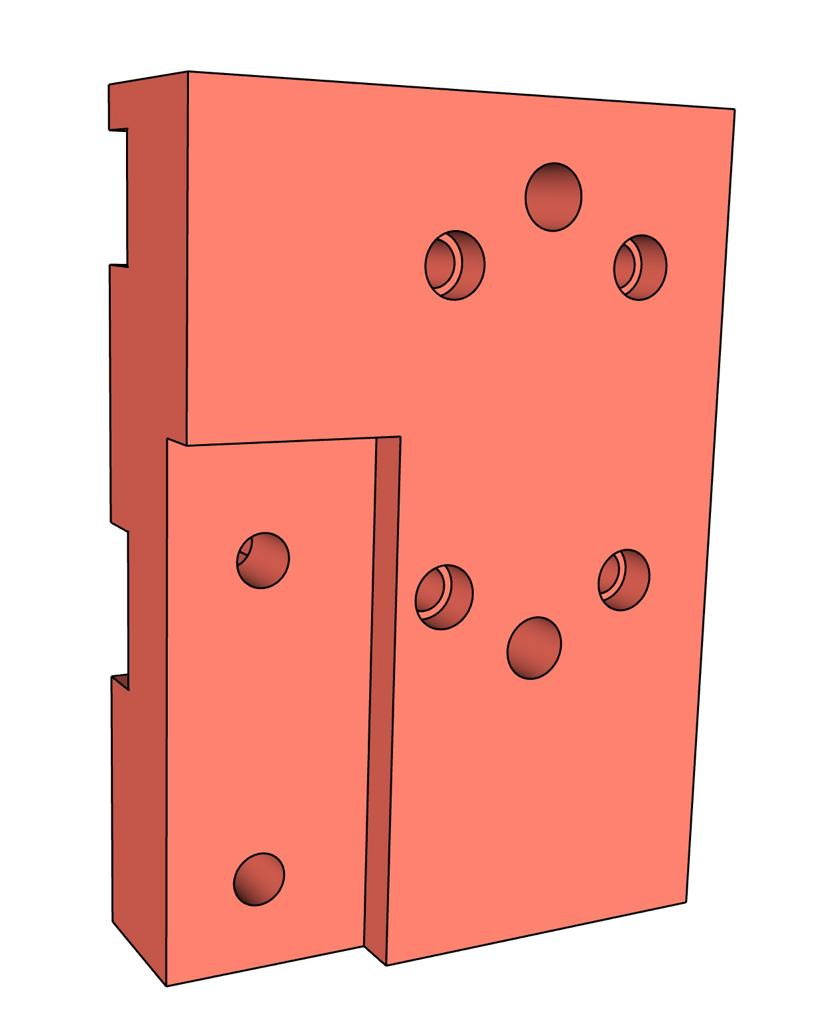
\includegraphics[scale = 0.4]{figuras/ressuportehastemancalf}
\caption{Suporte da haste e mancal vista da frente.}
\caption*{Fonte: Próprio autor}
\label{fig:ressuportehastemancalf}
\end{figure}
%\end{landscape}

% LANDSCAPE  - width = 0.4\linewidth
% LANDSCAPE  - scale = 0.30
% NORMAL  - width = 0.7\linewidth
% NORMAL  - scale = 0.45 a que eu mais gostei
%\begin{landscape}
\begin{figure}[H]
\centering
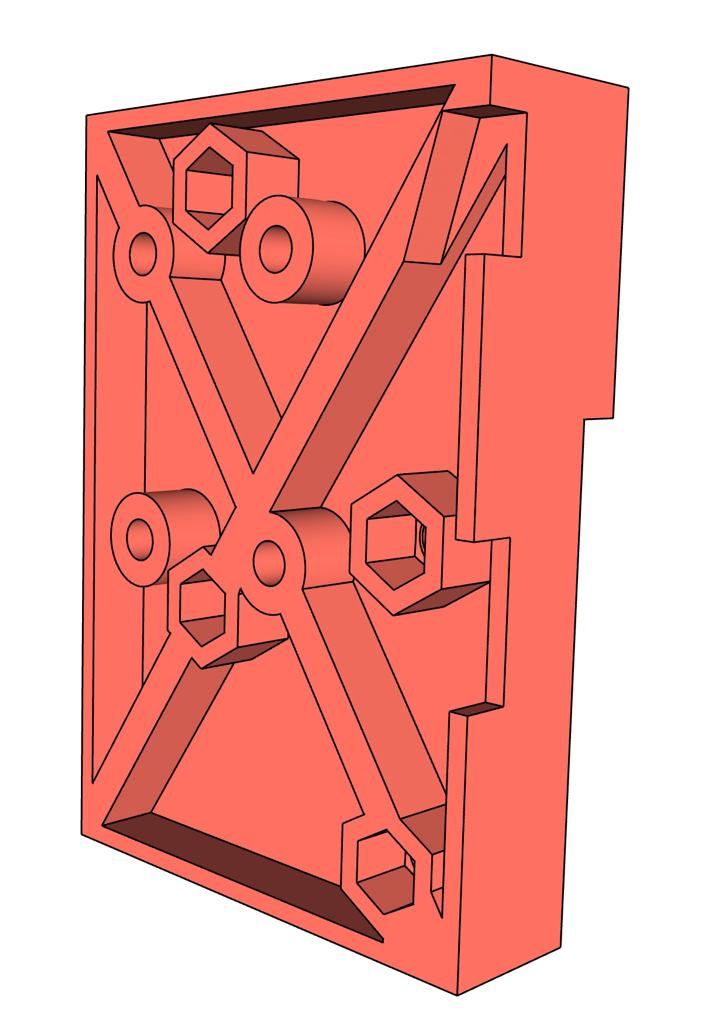
\includegraphics[scale = 0.4]{figuras/ressuportehastemancalfv}
\caption{Suporte da haste e mancal vista do verso.}
\caption*{Fonte: Próprio autor}
\label{fig:ressuportehastemancalfv}
\end{figure}
%\end{landscape}
        
% LANDSCAPE  - width = 0.4\linewidth
% LANDSCAPE  - scale = 0.30
% NORMAL  - width = 0.7\linewidth
% NORMAL  - scale = 0.45 a que eu mais gostei
%\begin{landscape}
\begin{figure}[H]
\centering
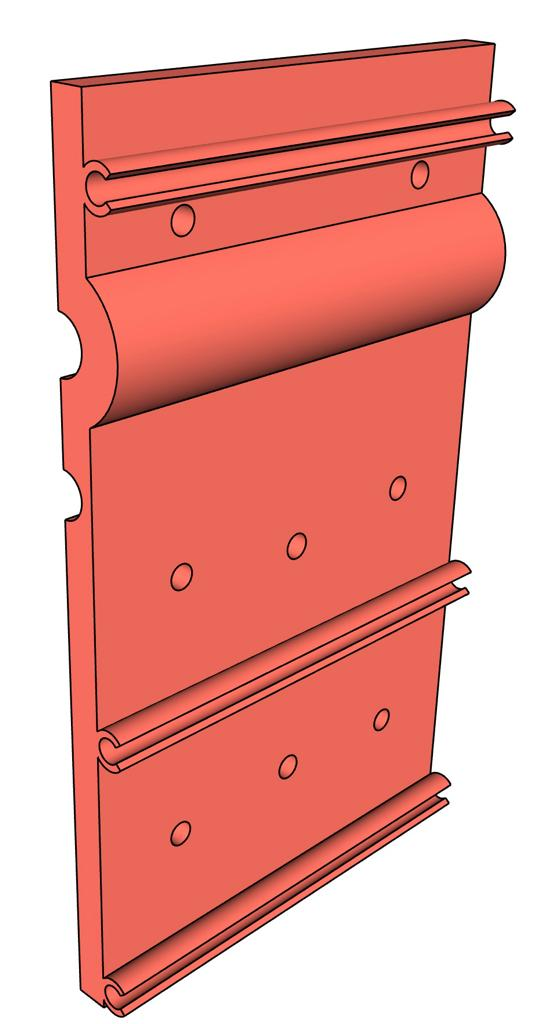
\includegraphics[scale = 0.4]{figuras/ressuporteservicofrontalf}
\caption{Suporte do serviço frontal vista da frente.}
\caption*{Fonte: Próprio autor}
\label{fig:ressuporteservicofrontalf}
\end{figure}
%\end{landscape}
        
% LANDSCAPE  - width = 0.4\linewidth
% LANDSCAPE  - scale = 0.30
% NORMAL  - width = 0.7\linewidth
% NORMAL  - scale = 0.45 a que eu mais gostei
%\begin{landscape}
\begin{figure}[H]
\centering
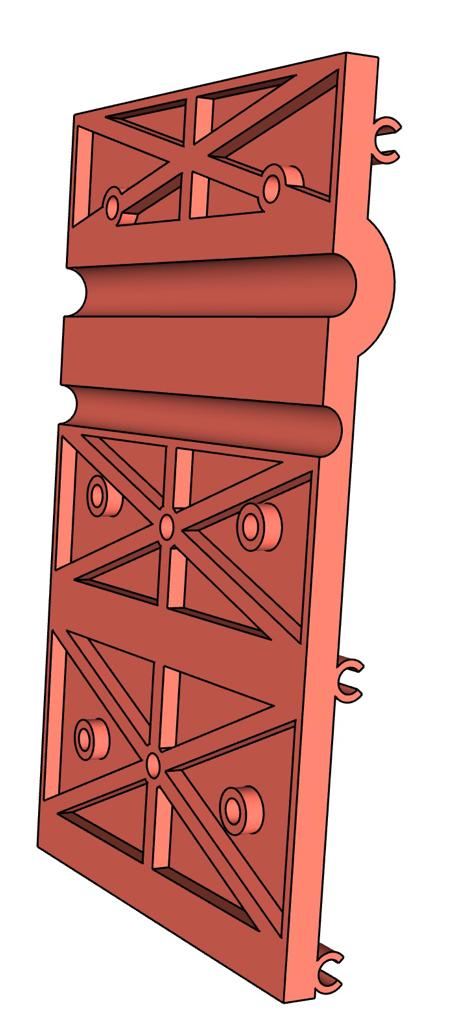
\includegraphics[scale = 0.4]{figuras/ressuporteservicofrontalfv}
\caption{Suporte do serviço frontal vista do verso.}
\caption*{Fonte: Próprio autor}
\label{fig:ressuporteservicofrontalfv}
\end{figure}
%\end{landscape}

% LANDSCAPE  - width = 0.4\linewidth
% LANDSCAPE  - scale = 0.30
% NORMAL  - width = 0.7\linewidth
% NORMAL  - scale = 0.45 a que eu mais gostei
%\begin{landscape}
\begin{figure}[H]
\centering
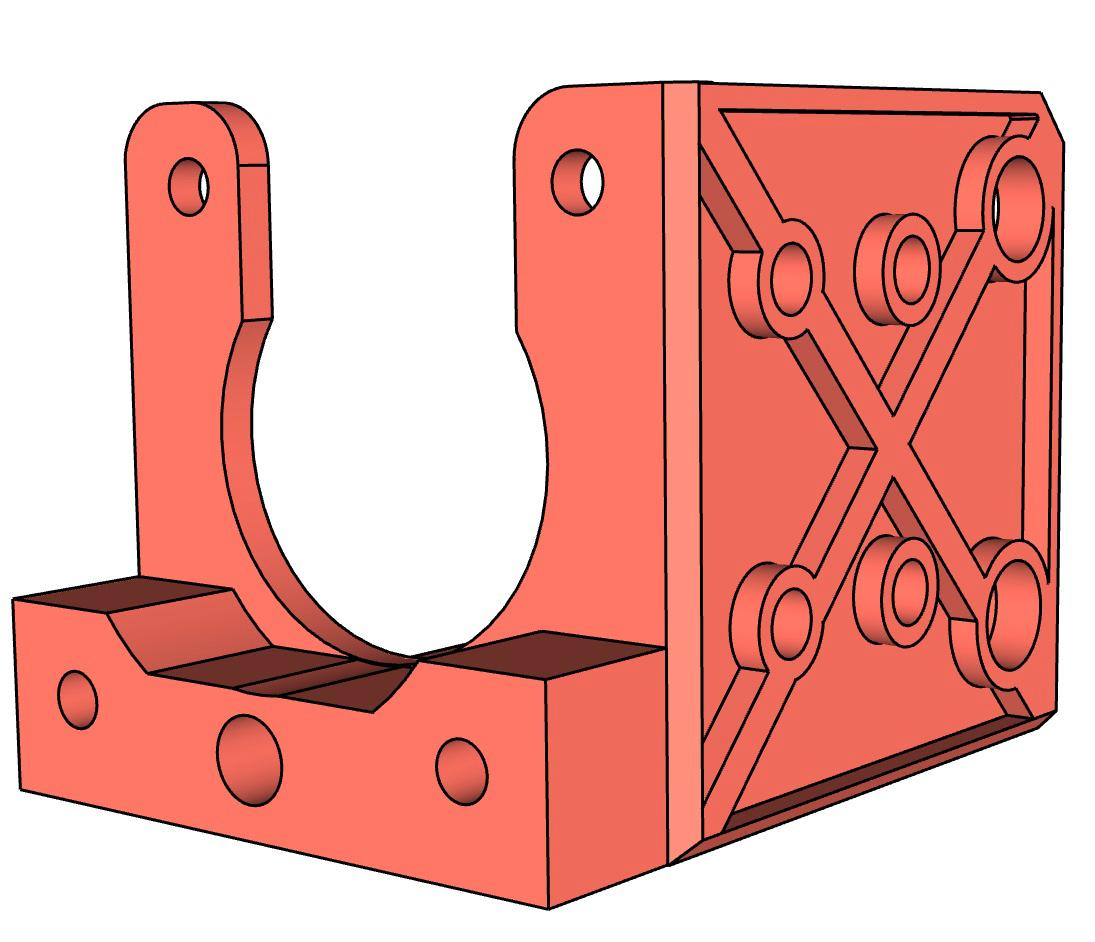
\includegraphics[scale = 0.4]{figuras/ressuportemotorhorizontalf}
\caption{Suporte do motor horizontal vista frontal.}
\caption*{Fonte: Próprio autor}
\label{fig:ressuportemotorhorizontalf}
\end{figure}
%\end{landscape}

% LANDSCAPE  - width = 0.4\linewidth
% LANDSCAPE  - scale = 0.30
% NORMAL  - width = 0.7\linewidth
% NORMAL  - scale = 0.45 a que eu mais gostei
%\begin{landscape}
\begin{figure}[H]
\centering
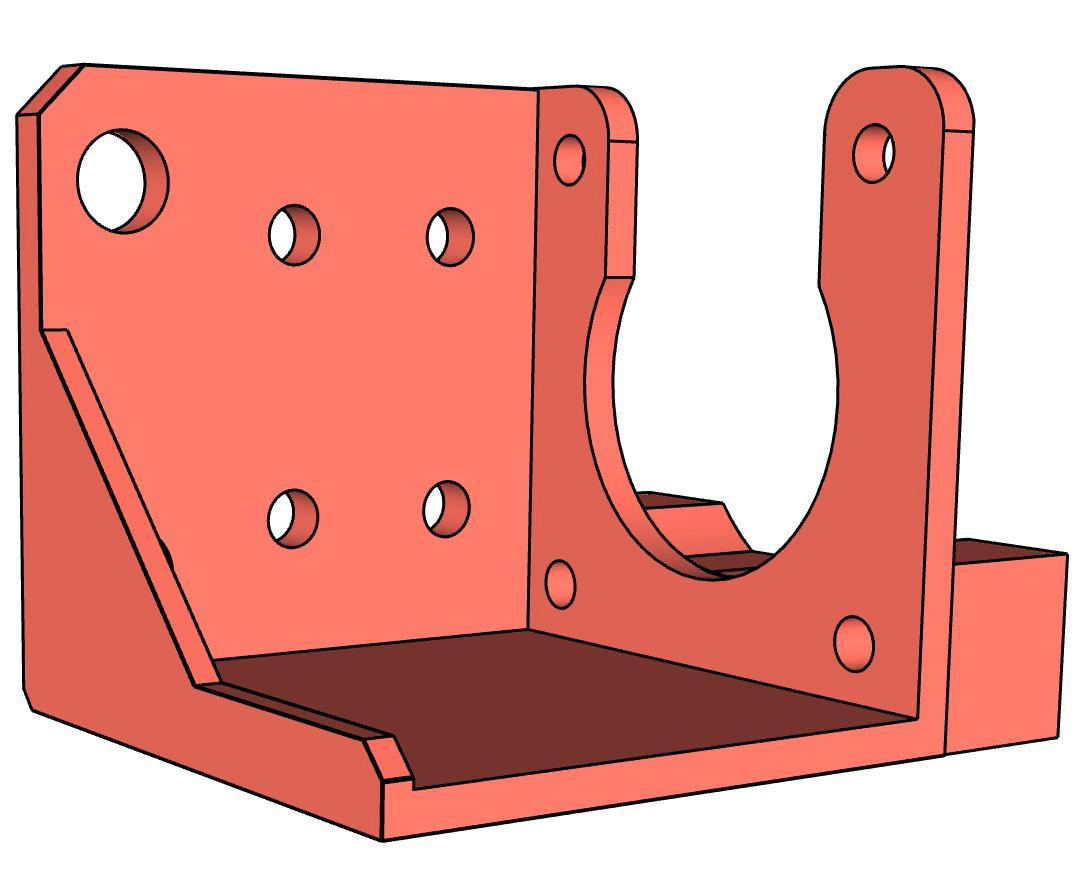
\includegraphics[scale = 0.4]{figuras/ressuportemotorhorizontalfv}
\caption{Suporte do motor horizontal vista frontal.}
\caption*{Fonte: Próprio autor}
\label{fig:ressuportemotorhorizontalfv}
\end{figure}
%\end{landscape}
        

\section{Sistema eletrônico}\label{sec:ressisele}

A Figura X mostra um esquema elétrico que comanda os motores de passos presentes na estrutura  da mesa 
cartesiana possibilitando uma melhor compreensão do funcionamento dos seus componentes.

%
%
%COLOCAR A IMAGEM DO ESQUEMA ELÉTRICO AQUI QUE DA PARA FAZER PELO TINKERCAD.COM


\section{Sistema de software}\label{sec:ressissof}

O sistema de software do projeto foi fundamentado na metodologia, sendo assim para o desenvolvimento 
do código foi utilizado a plataforma de prototipação Arduino IDE respeitando o diagrama de classes 
mostrado na seção 3.3.3.

A seguir serão mostrados os arquivos header de cada classe presente no sistema a fim de resumir 
o código fonte da sua versão completa. Esta versão se encontra nos apêndices do trabalho.

%HEADER DA CLASSE PINO
\subsection{Código header da classe Pino}\label{subsec:respino}

Segue abaixo o arquivo header (Pino.h) da classe “Pino”.

{\lstinputlisting[
    language        = C++,
    morekeywords    = {Driver, Eixo, Pino, Sigmoidal},
    style           = mystyle
]{elementos-pos-textuais/apendices/Pinoh.txt}

%OBJETO DA CLASSE PINO
Assim para se utilizar as funções presentes na classe “Pino” é criado um objeto 
através do comando abaixo com seus devidos parâmetros de entrada.

\lstinputlisting[style = mystyle]{elementos-pos-textuais/apendices/Pinoobj.txt}

%HEADER DA CLASSE SIGMOIDAL
\subsection{Código header da classe Sigmoidal}\label{subsec:ressigmoidal}

Segue abaixo o arquivo header (Sigmoidal.h) da classe “Sigmoidal”.

\lstinputlisting[style = mystyle]{elementos-pos-textuais/apendices/Sigmoidalh.txt}

%OBJETO DA CLASSE SIGMOIDAL
Assim para se utilizar as funções presentes na classe “Sigmoidal” é criado um objeto 
através do comando abaixo com seus devidos parâmetros de entrada.

\lstinputlisting[style = mystyle]{elementos-pos-textuais/apendices/Sigmoidalobj.txt}

%HEADER DA CLASSE DRIVER
\subsection{Código header da classe Driver}\label{subsec:resdriver}
Segue abaixo o arquivo header (Driver.h) da classe “Driver”.

\lstinputlisting[style = mystyle]{elementos-pos-textuais/apendices/Driverh.txt}

%OBJETO DA CLASSE DRIVER
Para flexibilização na utilização de diferentes tipos de drivers, foi desenvolvido 
duas construções diferentes para utilizar as funções da classe “Driver”.

%OBJETO 1 CLASSE DRIVER
A primeira é passando como parâmetros o pino do passo e da direção como no código abaixo.
Essa construção é para drivers que se responsabilizam pelo controle do estado 
das bobinas através do seu hardware.

\lstinputlisting[style = mystyle]{elementos-pos-textuais/apendices/Driverobj.txt}

%OBJETO 2 CLASSE DRIVER
Já a segunda é passando como parâmetros os pinos das bobinas como no código abaixo.
Essa construção é para drivers que terceirizam para o software o controle
do estado das bobinas.

\lstinputlisting[style = mystyle]{elementos-pos-textuais/apendices/Driverobj2.txt}

%HEADER DA CLASSE EIXO
\subsection{Código header da classe Eixo}\label{subsec:reseixo}

Segue abaixo o arquivo header (Eixo.h) da classe “Eixo”.

\lstinputlisting[style = mystyle]{elementos-pos-textuais/apendices/Eixoh.txt}

%OBJETO DA CLASSE EIXO
Assim para se utilizar as funções presentes na classe “Eixo” é criado um objeto 
através do comando abaixo com seus devidos parâmetros de entrada.

\lstinputlisting[style = mystyle]{elementos-pos-textuais/apendices/Eixoobj.txt}

%EXPLICANDO COMO A MESACARTESIANA.INO FUNCIONA
\subsection{Detalhamento do arquivo principal (MesaCartesiana.ino)}\label{subsec:resmesa}

O arquivo principal tem a responsabilidade de gerenciar toda aplicação, neste arquivo 
serão construídos todos objetos necessários. Segue abaixo um resumo com todas 
funcionalidades que este possui.

\lstinputlisting[style = mystyle]{elementos-pos-textuais/apendices/MesaCartesianaino.txt}

O método “incializarEixos” é responsável por construir os objetos necessários para controle dos 
eixos da aplicação, neste é possível escolher se o tipo de acionamento do driver 
é via software ou hardware.

O método “interpretarComandos” é responsável pela interpretação de qual comando foi enviado pelo usuário,
como por exemplo o comando “MOVER 2,4” que movimenta o eixo X para a ordenada 2 e o eixo Y para a ordenada 4.
Outros comandos necessários para uma aplicação como a mudança de estados de algumas configurações 
devem ser interpretadas por este método.

O método “movimentarMesa” é responsável pela chamada da funcionalidade de rotação presente na classe “Eixo” 
para isso recebe como parâmetro a coordenada enviada pelo usuário.

O método “escolherModoPasso” é responsável por setar qual o modo do passo que o eixo irá operar.

O método “setup” é responsável pela inicialização de toda aplicação estando nele uma chamada 
para o método de inicialização dos eixos.

O método “serialEvent” é responsável pela recepção dos dados enviados pelo usuário estando nele uma chamada 
para o método de interpretação de comandos.

O método “loop” é responsável pela execução da aplicação de forma que ela nunca acabe, já que é necessário 
que o método “serialEvent” esteja sempre em operação para quando o usuário solicitar alguma ação no sistema 
esta seja executada.